\documentclass[a0,portrait]{a0poster}

\usepackage[utf8]{inputenc}
\usepackage{multicol}
\usepackage[svgnames]{xcolor}
\usepackage{times}
\usepackage{graphicx}
\usepackage{booktabs}
\usepackage{array}
\usepackage{amsmath,amssymb}
\usepackage[font=small,labelfont=bf]{caption}

\newcolumntype{L}[1]{>{\raggedright\arraybackslash}p{#1}}

\graphicspath{{../pages/assets/}{figures/}}
\columnsep=90pt
\columnseprule=2pt

\definecolor{PosterBlue}{RGB}{35,78,112}
\definecolor{PosterOrange}{RGB}{217,107,43}
\definecolor{PosterText}{RGB}{42,47,52}
\definecolor{PosterLight}{RGB}{246,242,235}

\begin{document}

% -----------------------------------------------------------------------------
% Header
% -----------------------------------------------------------------------------

\begin{minipage}[b]{0.77\linewidth}
  \veryHuge\color{PosterBlue}\textbf{Geospatial Proximity Engine}\color{Black}\\[0.8cm]
  \Huge\textit{Exact network-distance classification through safe candidate screening}\\[1.4cm]
  \huge\textbf{Abrahim Borgi, Senior Business Analyst}
\end{minipage}
\begin{minipage}[b]{0.21\linewidth}
  \raggedleft
  
\includegraphics[width=14cm]{logo.png}
\end{minipage}

\vspace{1.2cm}
\hrule height 3pt
\vspace{1.2cm}

\begin{multicols}{2}
\color{PosterText}
\large

% -----------------------------------------------------------------------------
% Problem
% -----------------------------------------------------------------------------

\section*{Problem}

Many decisions require classifying which target locations are within a radius of
one or more sources. Straight-line distance is insufficient when access depends
on roads, paths, barriers, one-way restrictions or a selected travel profile.

The objective is therefore to identify source--target pairs whose shortest
directed network distance is at most a radius $r$, and then summarize the
accepted targets by count and weight. The radius may be stated in routed metres
or duration; for a time radius, an assumed average movement speed supports
candidate screening while OSRM evaluates the actual travel time.

\begin{center}
  \begin{minipage}[t]{0.48\linewidth}
    \centering
    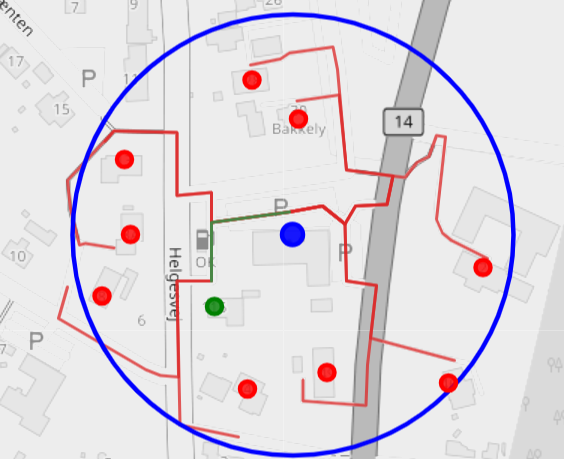
\includegraphics[width=\linewidth,height=18cm,keepaspectratio]{model2image.png}
  \end{minipage}\hfill
  \begin{minipage}[t]{0.48\linewidth}
    \centering
    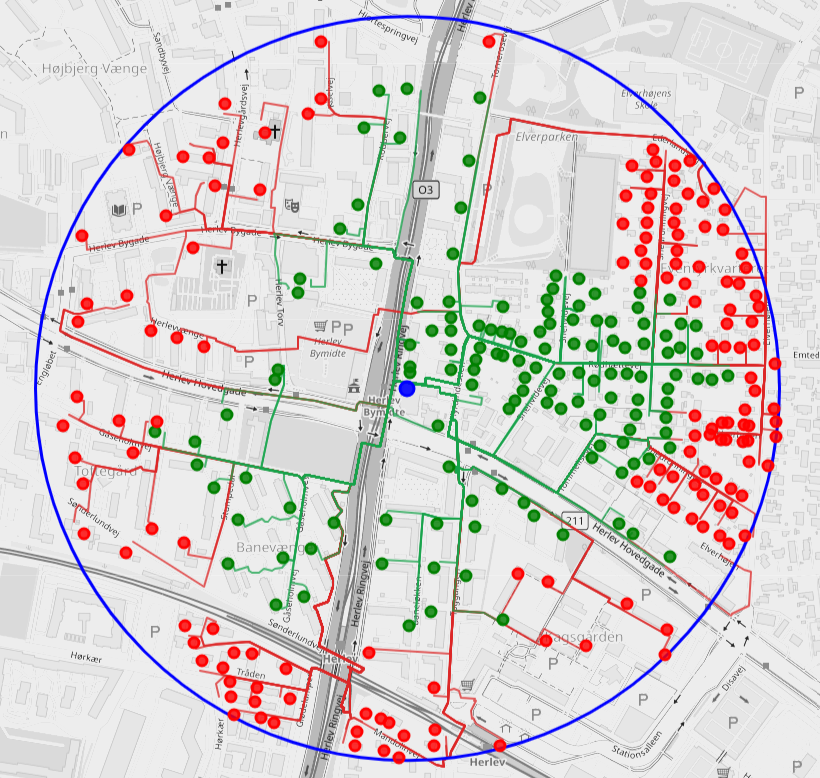
\includegraphics[width=\linewidth,height=18cm,keepaspectratio]{frontpage.png}
  \end{minipage}
  \captionof{figure}{Sources, targets and the routed network define the proximity classification problem.}
\end{center}
\vspace{-1.2cm}

% -----------------------------------------------------------------------------
% Theory
% -----------------------------------------------------------------------------

\section*{Theory}

Let $G=(V,E,w)$ be a directed travel graph with non-negative edge lengths.
Sources are $S=(s_1,\ldots,s_m)$ and targets are
$T=(t_1,\ldots,t_n)$. The routed distance is the directed shortest-path
distance $d_G(s_i,t_j)$.

For radius $r\geq0$, the accepted relation is
\[
  R_r=\{(i,j):d_G(s_i,t_j)\leq r\}.
\]

Let $\delta(s,t)$ denote great-circle distance. For every feasible path
$P=(v_0=s,\ldots,v_k=t)$, the triangle inequality gives
\[
  \delta(s,t)
  \leq \sum_{\ell=1}^{k}\delta(v_{\ell-1},v_\ell)
  \leq \sum_{\ell=1}^{k}w(v_{\ell-1},v_\ell).
\]
Minimizing over all feasible paths yields
\[
  \delta(s,t)\leq d_G(s,t).
\]

Consequently, $\delta(s,t)>r$ implies $d_G(s,t)>r$. Such a pair cannot
be accepted and may be removed before routing. Candidate screening is therefore
exact: it reduces OSRM work without removing any true network-distance match.

\begin{center}
  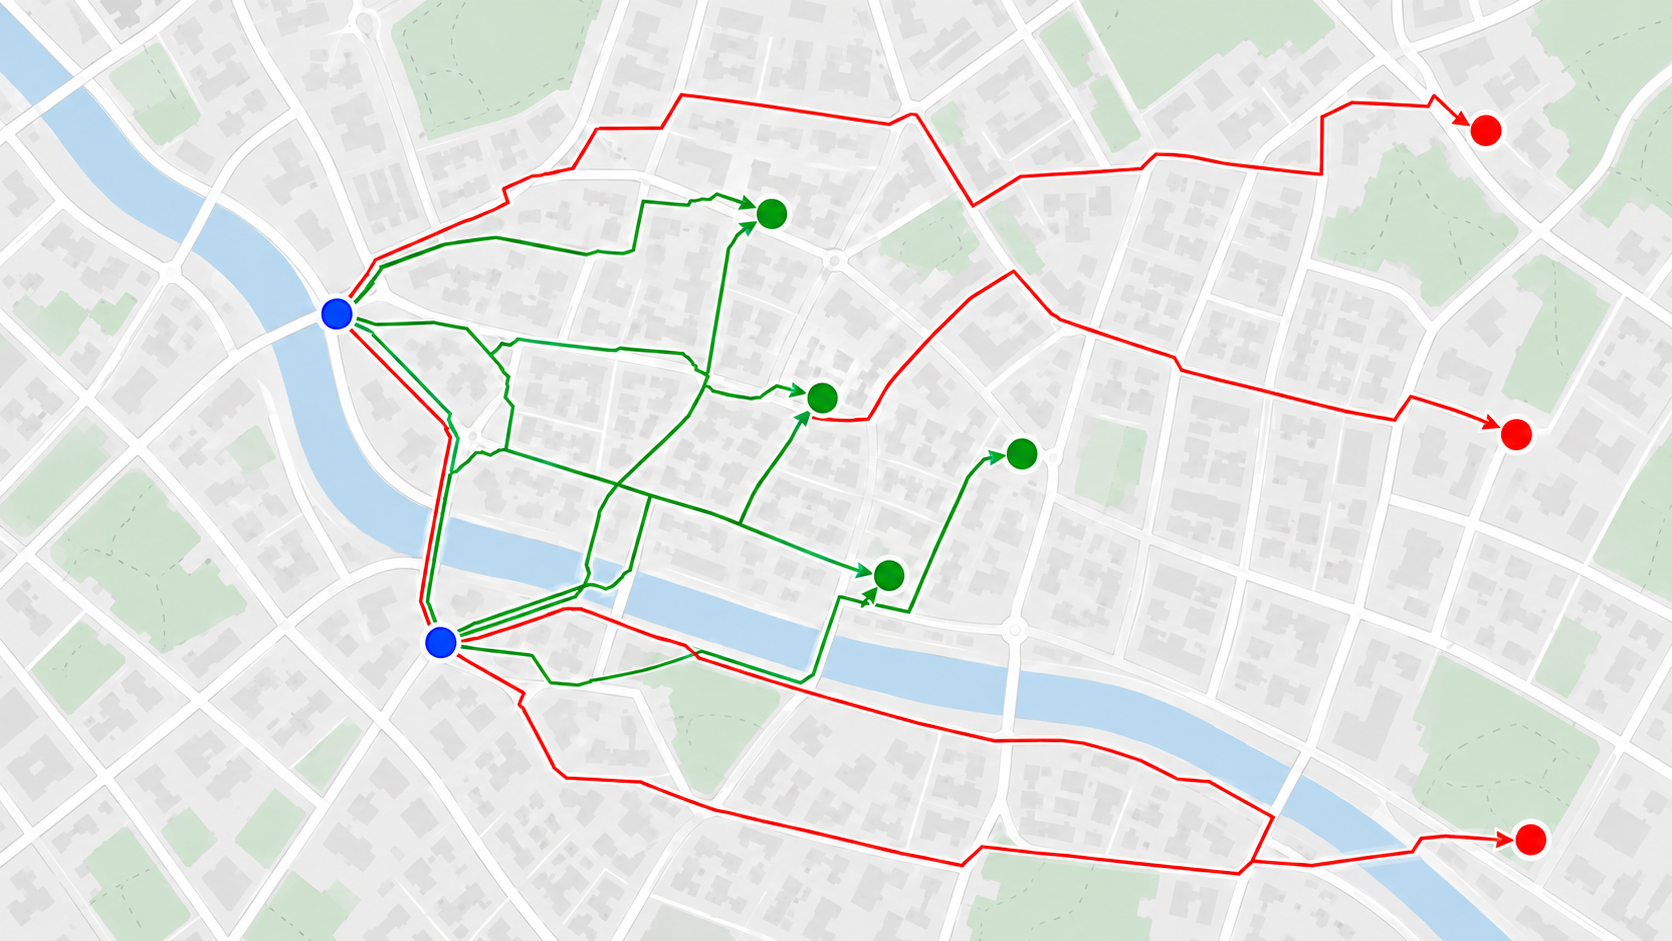
\includegraphics[width=0.96\linewidth,height=14cm,keepaspectratio]{theory_network.png}
  \captionof{figure}{Road-following relations from two sources to accepted and rejected candidates.}
\end{center}

\columnbreak

% -----------------------------------------------------------------------------
% Algorithm
% -----------------------------------------------------------------------------

\section*{Four-Step Algorithm}

\begin{enumerate}
  \item \textbf{Candidate selection.}
  Retain $(i,j)$ only when the geographic lower bound satisfies
  $\delta(s_i,t_j)\leq r$.

  \item \textbf{Directed distance calculation.}
  Use OSRM to evaluate $D_{ij}=d_G(s_i,t_j)$ for candidate pairs in the
  conceptual $m\times n$ source-to-target matrix.

  \item \textbf{Radius decision.}
  Accept candidate $(i,j)$ when $D_{ij}\leq r$; otherwise classify it as
  outside the routed radius.

  \item \textbf{Aggregation.}
  Return accepted-relation count, summed target weight, unique-target count and
  unique summed weight.
\end{enumerate}

The distinction between relation-based and unique measures is important. A
target reached from multiple sources contributes once per relation to the first
set of measures, but only once to unique geographic coverage.

% -----------------------------------------------------------------------------
% Implementation
% -----------------------------------------------------------------------------

\section*{Implementation}

The implementation separates mathematical screening from network routing.
Python controls the workflow, while OSRM evaluates directed shortest paths for
the selected travel profile.

\begin{center}
\begin{tabular}{L{0.22\linewidth} L{0.37\linewidth} L{0.29\linewidth}}
\toprule
\textbf{Component} & \textbf{Responsibility} & \textbf{Output} \\
\midrule
Preprocessing & Validate coordinates and weights; compute the Haversine lower bound & Candidate index pairs \\
Distance engine & Query OSRM Table in bounded chunks while preserving direction & Source-to-target distance blocks \\
Classification & Apply the radius rule and aggregate accepted relations & Matrix, counts and weighted summaries \\
Visualisation & Request OSRM route geometry and render it with Folium & Interactive route map \\
\bottomrule
\end{tabular}
\captionof{table}{Implementation responsibilities and data products.}
\end{center}

The computational interface returns a NumPy distance matrix, explicit accepted
relations and both relation-based and unique weighted summaries. The same code
supports walking, driving and cycling by changing only the OSRM profile, with
the radius expressed either as distance or duration.

% -----------------------------------------------------------------------------
% Applications
% -----------------------------------------------------------------------------

\section*{Applications}

The engine is a reusable classification component. Business meaning is supplied
through the choice of sources, targets, travel profile, radius and target weight.

\begin{center}
\begin{tabular}{L{0.23\linewidth} L{0.29\linewidth} L{0.36\linewidth}}
\toprule
\textbf{Use case} & \textbf{Sources} & \textbf{Decision output} \\
\midrule
Address coverage & Candidate sites & Reachable addresses and weighted potential \\
Competitive context & Own or proposed stores & Comparable stores within $n$ routed metres \\
Lead classification & Lead locations & Nearby targets, unique coverage and total weight \\
Service planning & Depots or facilities & Network-accessible demand by travel profile \\
\bottomrule
\end{tabular}
\captionof{table}{Representative applications of the same source--target relation.}
\end{center}

% -----------------------------------------------------------------------------
% Contribution
% -----------------------------------------------------------------------------

\section*{Contribution}

\begin{itemize}
  \item Exact candidate pruning justified by the triangle inequality.
  \item Directed route-distance classification rather than circular buffering.
  \item Scalable OSRM table queries restricted to viable candidates.
  \item Relation-based and unique weighted summaries for decision support.
  \item A reusable implementation across sites, stores, addresses and leads.
\end{itemize}

\color{PosterOrange}
\section*{Key Message}

\Large
Geographic distance provides a safe lower bound; network distance makes the
decision. The combination preserves exactness while avoiding unnecessary routing
queries.

\end{multicols}
\end{document}
